\documentclass[11pt]{scrartcl}
\usepackage[sexy]{evan}
\usepackage{graphicx}
\graphicspath{ {./images/} }

\usepackage{answers}
\Newassociation{hint}{hintitem}{all-hints}
\renewcommand{\solutionextension}{out}
\renewenvironment{hintitem}[1]{\item[\bfseries #1.]}{}

\usepackage{venndiagram,multicol,hyperref,graphicx,array}

\begin{document}
\title{Principio de Casillas}
\author{Ricardo Largaespada}
\date{27 Abril 2024}

\maketitle
\section{Introducción}
En esta clase continuaremos practicando las ideas de la clase anterior, aplicando el principio de la casa de los puntos en problemas más sofisticados y en algunos tipos de problemas que llamaremos problemas de coloración.

\begin{example}
Cada casilla de un tablero \(3 \times 7\) se pinta de negro o blanco. Muestra que es posible encontrar un rectángulo (con lados paralelos a los del tablero) cuyos cuatro puntos son del mismo color.
\end{example}
Solución. Cada columna de este tablero puede ser pintada de una de las siguientes formas:
\begin{center}
    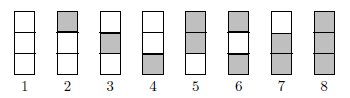
\includegraphics[scale=1]{images/clase_08_coloreo.png}
\end{center}
Observa que si la pintura 1 es elegida, bastaría una columna del tipo 2, 3 o 4 para formar un rectángulo. Con esto, nos quedan solo otras cuatro pinturas, pero tenemos siete columnas. Por lo tanto, por el principio de casillas, tendríamos dos columnas iguales. Lo mismo ocurre con la columna del tipo 8.\\

Ahora supongamos que ninguna de las columnas es del tipo 1 o 8. De esta manera, quedarían solo 6 tipos de pinturas. Así, por el principio de casillas, dos de ellas serían iguales.

\begin{example}[Bielorusia, 2007]
    Los puntos de un plano se pintan usando tres colores. Demuestra que existe un triángulo isósceles monocromático.
\end{example}
Solución. Supongamos que existe una forma de pintar el plano de modo que no exista un triángulo isósceles monocromático. Supongamos sin pérdida de generalidad que el centro O sea verde. De esta manera, puede haber como máximo un único punto verde entre los puntos del círculo. Así, es posible construir un pentágono regular \(A_1A_2A_3A_4A_5\) cuyos vértices son todos azules o rojos.

Entonces, por el principio de casillas, existirán tres vértices del pentágono que serán del mismo color. Y como cualquier tres vértices de un pentágono regular forman un triángulo isósceles, existirá un triángulo isósceles monocromático.

\begin{example}[Leningrado]
    Considera 70 enteros positivos distintos menores o iguales a 200. Demuestra que existen dos de ellos cuya diferencia es 4, 5 o 9.
\end{example}
Solución. Sean \(a_1, a_2, \ldots, a_{70}\) esos enteros positivos. Considera las siguientes listas:
\begin{align*}
\{a_1, a_2, \ldots, a_{70}\}; \\
\{a_1 + 4, a_2 + 4, \ldots, a_{70} + 4\}; \\
\{a_1 + 9, a_2 + 9, \ldots, a_{70} + 9\}.
\end{align*}
Tenemos un total de 210 números que están comprendidos entre 1 y 209 (inclusive). Por lo tanto, por el principio de casillas, existirán dos iguales. Como los números en la misma lista son siempre diferentes, será posible encontrar dos números en listas diferentes que sean iguales. Estos dos números satisfarán la condición del problema.

\begin{example}[Torneo de las ciudades 1998]
    En un tablero \(8 \times 8\), se marcan 17 casillas. Demuestra que es posible elegir dos de esas casillas marcadas de modo que un caballo de ajedrez necesite al menos tres movimientos para ir de una a otra.
\end{example}
Solución. Pinta las casillas del tablero usando 16 colores según la figura a continuación:
\[
\begin{matrix}
10 & 12 & 14 & 16 & 2 & 4 & 6 & 8 \\
10 & 12 & 14 & 16 & 2 & 4 & 6 & 8 \\
9 & 11 & 13 & 15 & 1 & 3 & 5 & 7 \\
9 & 11 & 13 & 15 & 1 & 3 & 5 & 7 \\
2 & 4 & 6 & 8 & 10 & 12 & 14 & 16 \\
2 & 4 & 6 & 8 & 10 & 12 & 14 & 16 \\
1 & 3 & 5 & 7 & 9 & 11 & 13 & 15 \\
1 & 3 & 5 & 7 & 9 & 11 & 13 & 15 \\
\end{matrix}
\]
Observa que para desplazarse entre dos casillas del mismo color, el caballo necesita al menos tres movimientos. Por lo tanto, por el principio de la casa de los puntos, entre 17 casillas marcadas, siempre habrá al menos dos del mismo color.

\begin{example}[Selectivo ConoSur,?]
    Los enteros \(1, 2, \ldots , 200\) se dividen en 50 conjuntos. Demuestra que al menos uno de esos 50 conjuntos contiene tres números distintos que pueden ser medidas de los lados de un mismo triángulo.    
\end{example}
Solución. Por el principio de casillas, entre los 101 enteros 100, 101, . . . , 200, al menos tres de ellos están en un mismo conjunto. Siendo \(a < b < c\) tales enteros, tenemos
\[ a + b \geq 100 + 101 = 201 > 200 \geq c \Rightarrow a + b > c, \]
y por lo tanto \(a\), \(b\) y \(c\) pueden ser medidas de los lados de un mismo triángulo.

\Opensolutionfile{all-hints}

\section{Problemas Propuestos}
\begin{problem}
Demuestra que para todo \(n > 1\) de cualquier subconjunto de \(n + 2\) elementos del conjunto \(1, 2, \ldots, 3n\) podemos elegir dos cuya diferencia es mayor que \(n\) y menor que \(2n\).
\end{problem}

\begin{problem}
En una zapatería hay 200 botas de talla 41, 200 botas de talla 42 y 200 botas de talla 43. De estas 600 botas, 300 son para el pie izquierdo y 300 para el derecho. Demuestra que existen al menos 100 pares de botas usables.
\end{problem}

\begin{problem}
Once estudiantes formaron cinco grupos de estudio. Demuestra que existen dos estudiantes A y B, tales que en todo grupo que incluye a A también incluye a B.
\end{problem}

\begin{problem}
Demuestra que si elegimos más de \(n\) números del conjunto \(\{1, 2, \ldots, 2n\}\), entonces uno de ellos será múltiplo de otro. ¿Puede esto evitarse con \(n\) números?
\end{problem}

\begin{problem}[Torneo das Cidades 1994]
Hay 20 alumnos en una escuela. Cualquier par de ellos comparte un abuelo común. Demuestra que al menos 14 de ellos tienen un abuelo en común.
\end{problem}

\begin{problem}[Rusia 1997]
Una sala de clases tiene 33 estudiantes. Cada estudiante tiene una canción y un cantante favorito. Un día, cada uno de ellos preguntó a los demás sobre sus canciones y cantantes favoritos. Luego, cada uno dijo dos números, el primero era la cantidad de estudiantes que les gustaba la misma canción y el segundo, la cantidad de estudiantes que tenían el mismo cantante favorito. Se sabe que cada uno de los números del 0 al 10 apareció entre las respuestas. Demuestra que existen dos estudiantes que les gusta el mismo cantante y la misma canción.
\end{problem}

\begin{problem}
Supón que para algún entero \(k \geq 1\), la suma de \(2k + 1\) enteros positivos distintos es menor que \((k + 1)(3k + 1)\). Demuestra que existen dos de ellos cuya suma es \(2k + 1\).
\end{problem}

\begin{problem}
¿Existe algún conjunto \(A\) formado por siete enteros positivos, ninguno de los cuales es mayor que 24, tal que las sumas de los elementos de cada uno de sus 127 subconjuntos no vacíos sean todas distintas par a par?
\end{problem}

\begin{problem}[USAMO 1985]
En una fiesta hay \(n\) personas. Demuestra que existen dos personas tales que, de las \(n - 2\) personas restantes, es posible encontrar \(\lfloor n/2 \rfloor - 1\) donde cada una de ellas conoce o no conoce a ambas.
\end{problem}

\begin{problem}
El plano está pintado usando dos colores. Demuestra que existen dos puntos del mismo color distantes exactamente un metro.
\end{problem}

\begin{problem}[Putnam]
El plano está pintado usando tres colores. Demuestra que existen dos puntos del mismo color distantes exactamente un metro.
\end{problem}

\begin{problem}
El plano está totalmente pintado usando dos colores. Demuestra que existe un rectángulo cuyos vértices son todos del mismo color.
\end{problem}

\begin{problem}[IMO 1983]
Cada punto del perímetro de un triángulo equilátero está pintado de uno de dos colores. Demuestra que es posible elegir tres puntos del mismo color formando un triángulo rectángulo.
\end{problem}

\begin{problem}
Nueve puntos de un icosaedro regular están pintados de rojo. Demuestra que podemos encontrar tres de ellos formando un triángulo isósceles.
\end{problem}

\begin{problem}[Rusia 2004]
Cada punto de coordenadas enteras está pintado de una de tres colores, siendo cada color usado al menos una vez. Demuestra que podemos encontrar un triángulo rectángulo cuyos vértices son de colores distintos.
\end{problem}

\begin{problem}
El plano está pintado usando tres colores. Demuestra que podemos encontrar un triángulo rectángulo isósceles con los tres vértices del mismo color.
\end{problem}


\Closesolutionfile{all-hints}

%\section{Sugerencias y Soluciones}
%\begin{enumerate}
%\input{all-hints.out}
%\end{enumerate}

\end{document}